\documentclass[tikz, border=10pt]{standalone}
\usetikzlibrary{automata, positioning, arrows}

\begin{document}

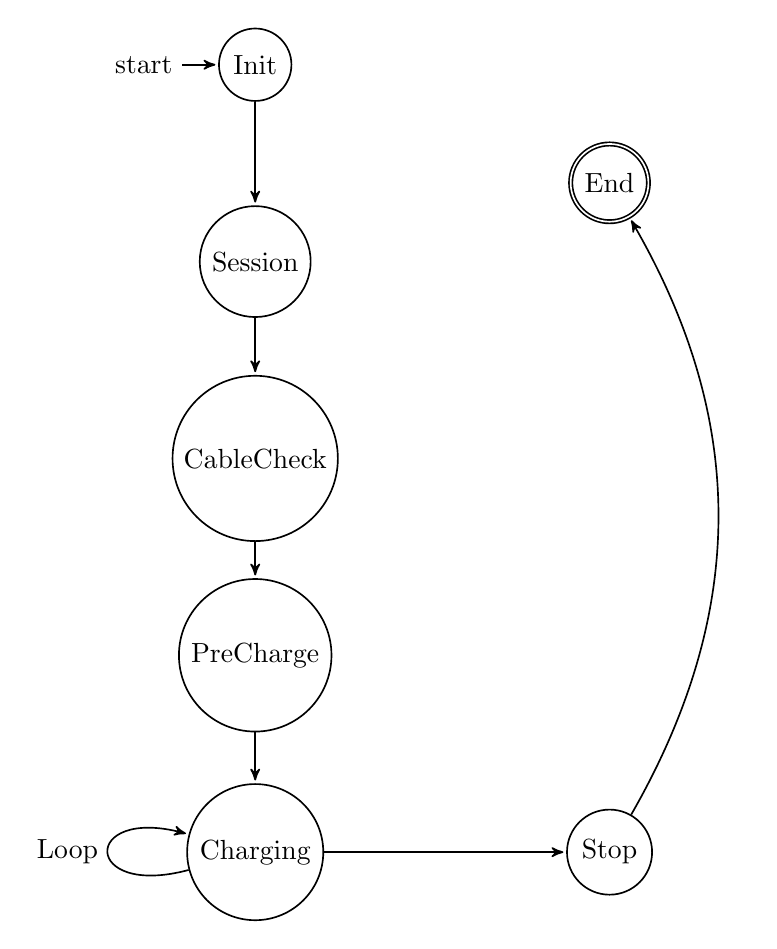
\begin{tikzpicture}[>=stealth', shorten >=1pt, auto, node distance=2.5cm, semithick]

  \tikzstyle{every state}=[fill=white, draw=black, text=black]

  \node[initial, state] (initial) {Init};
  \node[state] (Session) [below of=initial] {Session};
  \node[state] (CableCheck) [below of=Session] {CableCheck};
  \node[state] (PreCharge) [below of=CableCheck] {PreCharge};
  \node[state] (Charging) [below of=PreCharge] {Charging};
  \node[state] (Stop) [right of=Charging, xshift=2cm] {Stop};
  \node[state, accepting] (final) [above of=Stop, yshift=6cm] {End};

  \path[->] 
    (initial) edge node {} (Session)
    (Session) edge node {} (CableCheck)
    (CableCheck) edge node {} (PreCharge)
    (PreCharge) edge node {} (Charging)
    (Charging) edge node {} (Stop)
    (Stop) edge [bend right] node {} (final)
    (Charging) edge [loop left] node {Loop} (Charging);

\end{tikzpicture}

\end{document}
